%%%%%%%%%%%%%%%%%%%%%%%%%%%%%%%%%%%%%%%%%
% Beamer Presentation
% LaTeX Template
% Version 1.0 (10/11/12)
%
% This template has been downloaded from:
% http://www.LaTeXTemplates.com
%
% License:
% CC BY-NC-SA 3.0 (http://creativecommons.org/licenses/by-nc-sa/3.0/)
%
%%%%%%%%%%%%%%%%%%%%%%%%%%%%%%%%%%%%%%%%%

%----------------------------------------------------------------------------------------
%	PACKAGES AND THEMES
%----------------------------------------------------------------------------------------

\documentclass{beamer}

\mode<presentation> {

% The Beamer class comes with a number of default slide themes
% which change the colors and layouts of slides. Below this is a list
% of all the themes, uncomment each in turn to see what they look like.

%\usetheme{default}
%\usetheme{AnnArbor}
%\usetheme{Antibes}
%\usetheme{Bergen}
%\usetheme{Berkeley}
%\usetheme{Berlin}
%\usetheme{Boadilla}
%\usetheme{CambridgeUS}
%\usetheme{Copenhagen}
%\usetheme{Darmstadt}
%\usetheme{Dresden}
%\usetheme{Frankfurt}
%\usetheme{Goettingen}
%\usetheme{Hannover}
%\usetheme{Ilmenau}
%\usetheme{JuanLesPins}
%\usetheme{Luebeck}
\usetheme{Madrid}
%\usetheme{Malmoe}
%\usetheme{Marburg}
%\usetheme{Montpellier}
%\usetheme{PaloAlto}
%\usetheme{Pittsburgh}
%\usetheme{Rochester}
%\usetheme{Singapore}
%\usetheme{Szeged}
%\usetheme{Warsaw}

% As well as themes, the Beamer class has a number of color themes
% for any slide theme. Uncomment each of these in turn to see how it
% changes the colors of your current slide theme.

%\usecolortheme{albatross}
%\usecolortheme{beaver}
%\usecolortheme{beetle}
%\usecolortheme{crane}
%\usecolortheme{dolphin}
%\usecolortheme{dove}
%\usecolortheme{fly}
%\usecolortheme{lily}
%\usecolortheme{orchid}
%\usecolortheme{rose}
%\usecolortheme{seagull}
%\usecolortheme{seahorse}
%\usecolortheme{whale}
%\usecolortheme{wolverine}

%\setbeamertemplate{footline} % To remove the footer line in all slides uncomment this line
%\setbeamertemplate{footline}[page number] % To replace the footer line in all slides with a simple slide count uncomment this line

%\setbeamertemplate{navigation symbols}{} % To remove the navigation symbols from the bottom of all slides uncomment this line
}

\usepackage{graphicx} % Allows including images
\usepackage{booktabs} % Allows the use of \toprule, \midrule and \bottomrule in tables

%----------------------------------------------------------------------------------------
%	TITLE PAGE
%----------------------------------------------------------------------------------------

\title[Open SouRce. Summer Academy `15]{Introduction to open source Spatial Analysis Tools and R\\
\medskip \tiny{International Summer Academy on Spatial Ecotoxicology and Ecotoxicological Risk Assessment\\Using an Open Commmunity Approach}} % The short title appears at the bottom of every slide, the full title is only on the title page

\author[Avit Bhowmik]{Avit Kumar Bhowmik \\} % Your name
\institute[Uni Koblenz-Landau] % Your institution as it will appear on the bottom of every slide, may be shorthand to save space
{
Institute for Environmental Sciences, University of Koblenz-Landau \\ % Your institution for the title page
\medskip
\textit{bhowmik@uni-landau.de}% Your email address
}
\date{\today} % Date, can be changed to a custom date

\begin{document}

\begin{frame}
\titlepage % Print the title page as the first slide
\end{frame}

%------------------------------------------------

\begin{frame}
\frametitle{Who am I?}
\centering
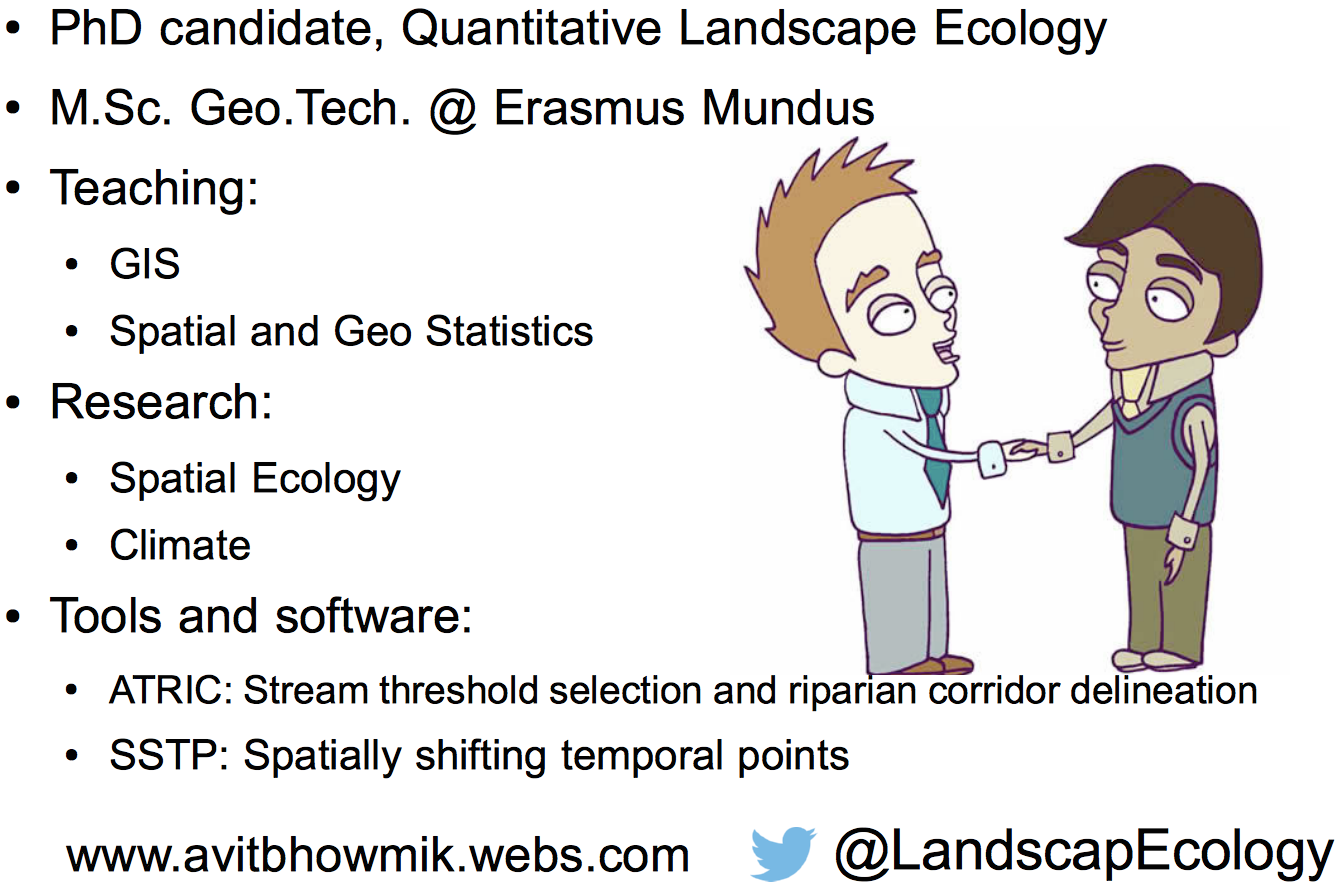
\includegraphics[width=0.95\textwidth]{Figures/Intro.png}
\end{frame}


%------------------------------------------------

\begin{frame}
\centering
\Huge ...and Gunnar
\end{frame}

%------------------------------------------------

\begin{frame}
\frametitle{Why Open Source?}
\centering
$\vcenter{\hbox{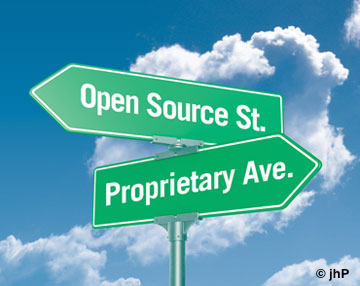
\includegraphics[width=0.28\textwidth]{Figures/op_vs_prp.png}}}$
\pause
$\vcenter{\hbox{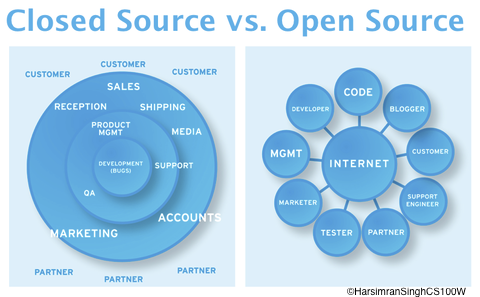
\includegraphics[width=0.7\textwidth]{Figures/Cls_vs_opn.png}}}$
\end{frame}

%-----------------------------------------------

\begin{frame}
\frametitle{Why Open Source?}
\begin{block}{Advantages}
\begin{itemize}
\item \alert{No costs (!!!)}\\
\small European Commision 2012: c.a. 450 billion euro savings p.a.
\href{https://joinup.ec.europa.eu/news/contribution-open-source-europes-economy-450-billion-year}{https://joinup.ec.europa.eu/news/contribution-open-source-europes-economy-450-billion-year}
\normalsize
\item \alert{Coherent standard with proprietary software}
\item \alert{Freedom to adjust and distribute program}
\item \alert{Transparency and Reproducibility}\\
\small Rocchini and Neteler (2012) TREE, Barnes (2010) Nature
\normalsize
\item \alert{Platform-independent}
\end{itemize}
\end{block}
\end{frame}

%-----------------------------------------------

\begin{frame}
\frametitle{Why Open Source?}
\begin{block}{(Dis)advantages}
\begin{itemize}
\item Comes without guarantee regarding bugs and features (but mailing lists and internet community) 
\item Sometimes smaller user communities (especially in companies and administration)
\item In most cases less user-friendly/steeper learning curve
\end{itemize}
\end{block}
\end{frame}

%-----------------------------------------------

\begin{frame}
\frametitle{Big communities of ``Free Open Source Software (FOSS)''}
\centering

\includegraphics[width=\textwidth]{Figures/FOSS.png}
\end{frame}

%-----------------------------------------------

\begin{frame}
\frametitle{Learn about ``Free Open Source Software (FOSS)''}
\centering
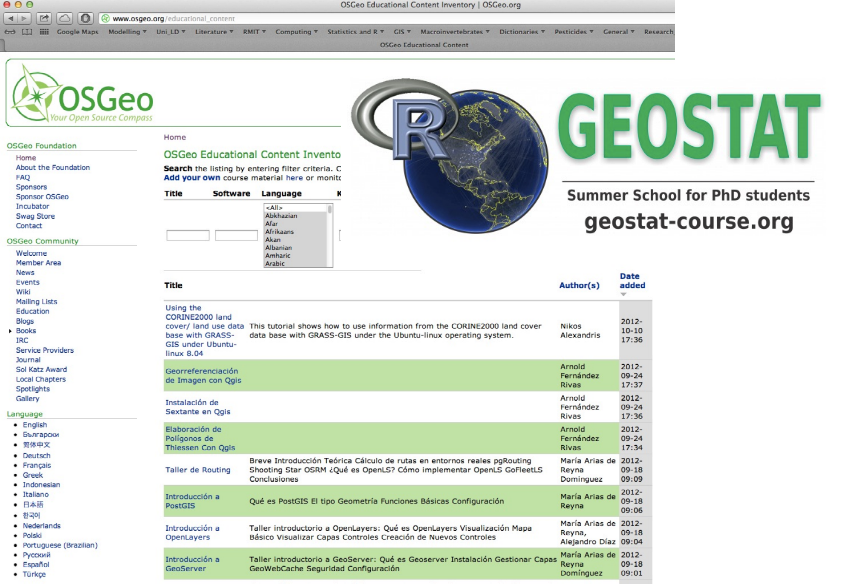
\includegraphics[width=\textwidth]{Figures/FOSS_ed.png}
\end{frame}

%-----------------------------------------------

\begin{frame}
\frametitle{Learn about ``Free Open Source Software (FOSS)''}
\centering
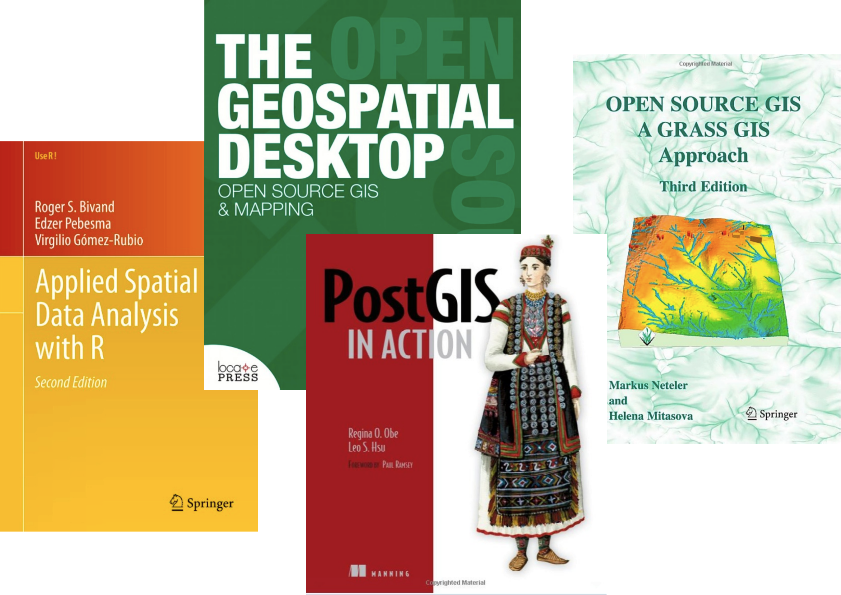
\includegraphics[width=\textwidth]{Figures/FOSS_books.png}
\end{frame}

%------------------------------------------------

\begin{frame}
\frametitle{Learn about ``Free Open Source Software (FOSS)''}
\centering
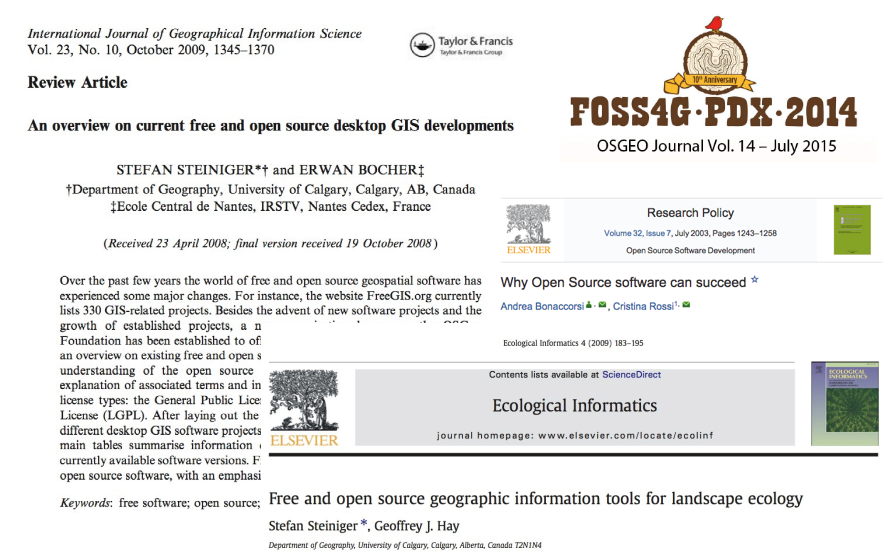
\includegraphics[width=\textwidth]{Figures/FOSS_articles.png}
\end{frame}

%------------------------------------------------

\begin{frame}
\frametitle{Open source (coherent) spatial analyses tools}
\centering
\begin{table}[h]
\begin{tabular}{p{3.0cm} p{4.0cm} p{4.0cm}}

\toprule

GIS Sector & Examples proprietary Software & Examples Free Open Source Software\\

\midrule

Desktop GIS & ArcGIS, GeoMedia, MapInfo, Idrisi & GRASS GIS, ILWIS, QGIS, SAGA GIS, \alert{R}\\[0.2cm]
Spatial Statistics & ArcGIS Extensions, Idrisi, ERDAS Imagine & OpenGeoDa, GeoMS, \alert{R \& packages} \\[0.2cm]
Spatial Databases & Oracle Spatial, ArcGIS SDE & PostGIS, SpatiaLite, \alert{R \& packages}\\[0.2cm]
Remote Sensing \& Image Processing & ERDAS Imagine, ENVI, Ecognition, IDL & OTB, ILWIS, Opticks, GRASS GIS, \alert{R}\\

\bottomrule

\end{tabular}
\end{table}
\end{frame}

%------------------------------------------------

\begin{frame}
\frametitle{R and moRe}
\centering

\includegraphics[width=0.3\textwidth]{Figures/Rlogo.png}
\pause
\begin{itemize}
\item R is a software (\alert{much more!}) for statistical (\alert{much much more!}) analyses
\pause
\item Syntax : C++ family
\pause
\item Object-oriented using classes
\pause
\item Originally available in command line interface, popular editor: \alert{RStudio}
\pause
\item Also available in graphical user interface (GUI), e.g. ``Duducer'' and ``R Commander''. \alert{But forget about them!}
\end{itemize}
\end{frame}

%------------------------------------------------

\begin{frame}
\frametitle{R and moRe}
\begin{block}{Why R?}
You cannot do it with anything else!
\end{block}
\pause
\centering
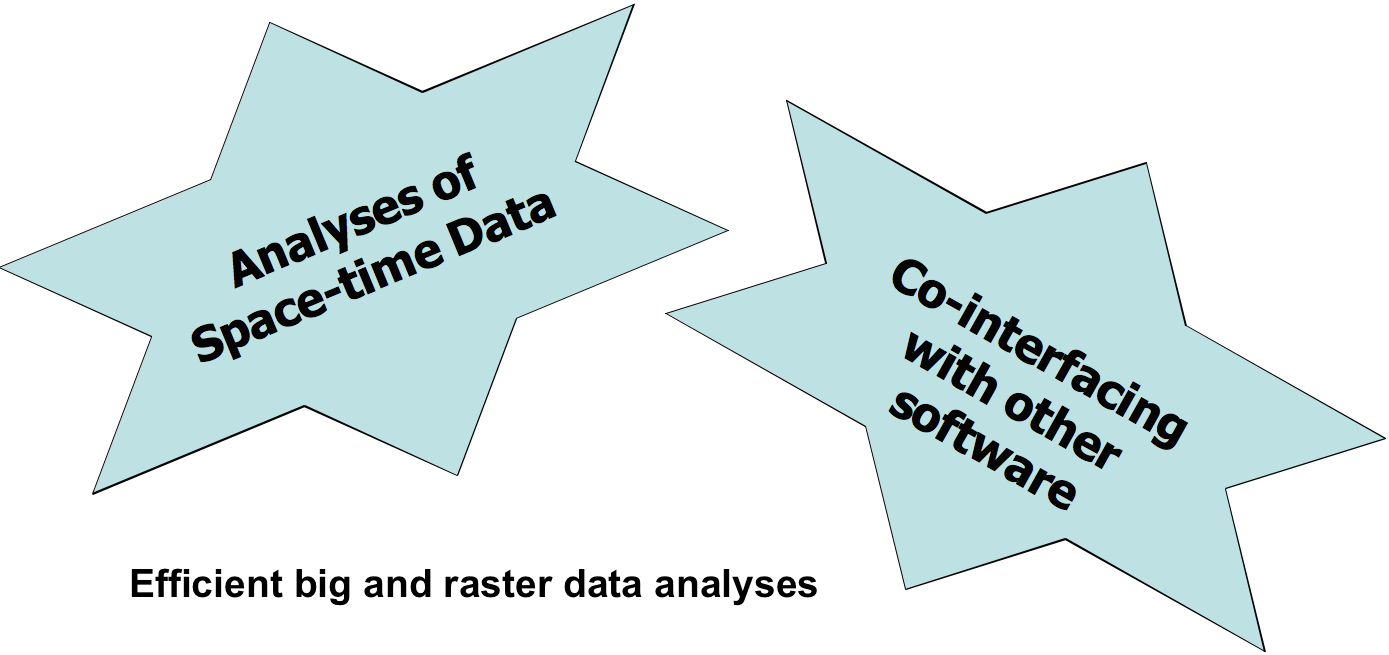
\includegraphics[width=\textwidth]{Figures/whyR.png}
\end{frame}

%------------------------------------------------

\begin{frame}
\frametitle{R and moRe: Functions}
\centering
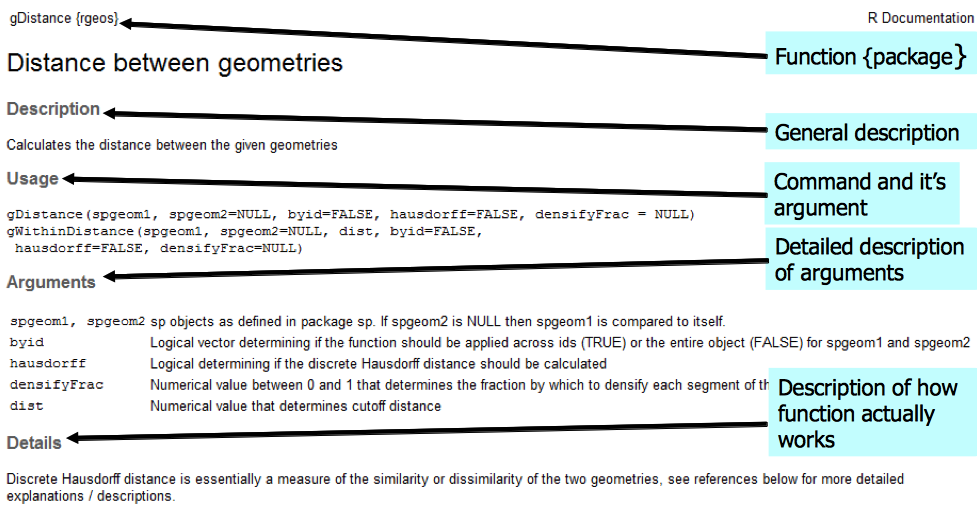
\includegraphics[width=\textwidth]{Figures/Rbasic1.png}
\end{frame}

%------------------------------------------------

\begin{frame}
\frametitle{R and moRe: Functions}
\centering
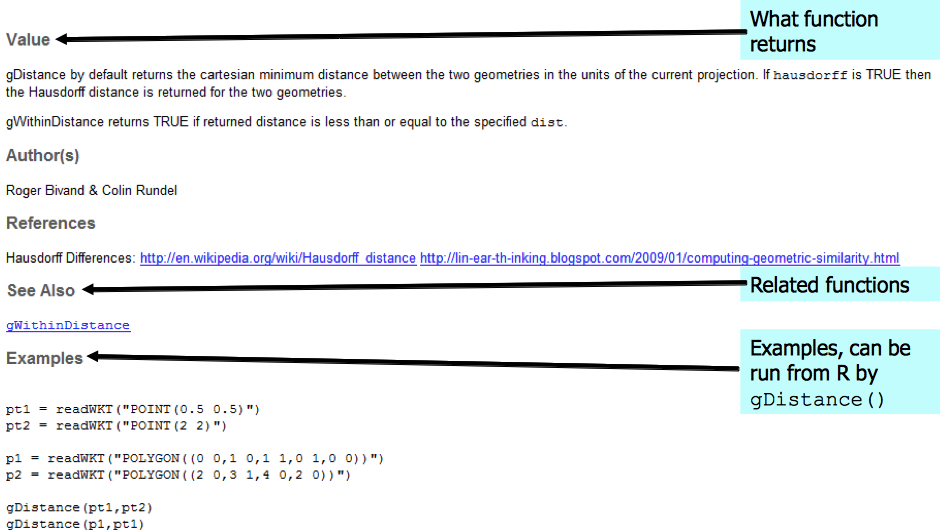
\includegraphics[width=\textwidth]{Figures/Rbasic2.png}
\end{frame}

%------------------------------------------------

\begin{frame}
\frametitle{R and moRe: Objects}
\begin{block}{Vector}
\begin{itemize}
\item An array (collection) of numbers, strings or factors
\item e.g. \alert{1 2 3 4 5} or \alert{``a'' ``b'' ``c'' ``d'' ``e''}
\end{itemize}
\end{block}
\vspace{1 cm}
\pause
\begin{block}{Factor}
\begin{itemize}
\item An array (collection) of level (grouping variables), can be numbers or strings
\item e.g. \alert{a b c d e}
\end{itemize}
\end{block}
\end{frame}

%------------------------------------------------


\begin{frame}
\frametitle{R and moRe: Objects}
\begin{block}{Matrix}
\begin{itemize}
\item A table where rows and columns contain vectors
\item Vector types of columns and rows should be the same, e.g. either numeric or string, these can not be combined 
\end{itemize}
\begin{tabular} {c c c}
 & \alert{col 1} & \alert{col 2}\\
\alert{row 1} & \alert{``a''} & \alert{``c''}\\
\alert{row 2} & \alert{``b''} & \alert{``d''}\\
\end{tabular}
\end{block}
\pause
\begin{block}{Data Frame}
\begin{itemize}
\item A table where columns contain vectors
\item Vector types of columns can be different, e.g. numeric and string, and can be combined 
\end{itemize}
\begin{tabular} {c c c}
 & \alert{vector 1} & \alert{vector 2}\\
\alert{row 1} & \alert{``a''} & \alert{1}\\
\alert{row 2} & \alert{``b''} & \alert{2}\\
\end{tabular}
\end{block}
\end{frame}

%------------------------------------------------

\begin{frame}
\frametitle{R and moRe: Objects}
\begin{block}{List}
\begin{itemize}
\item A collection of elements, vectors or other objects
\end{itemize}
List[[``Vector'']] \alert{``a'' ``b'' ``c'' ``d'' ``e''}\\
List[[``Matrix'']]\\
\begin{tabular} {c c c}
 & \alert{col 1} & \alert{col 2}\\
\alert{row 1} & \alert{``a''} & \alert{``c''}\\
\alert{row 2} & \alert{``b''} & \alert{``d''}\\
\end{tabular}\\
List[[``Data Frame'']]\\
\begin{tabular} {c c c}
 & \alert{vector 1} & \alert{vector 2}\\
\alert{row 1} & \alert{``a''} & \alert{1}\\
\alert{row 2} & \alert{``b''} & \alert{2}\\
\end{tabular}
\end{block}
\end{frame}

%------------------------------------------------

\begin{frame}[fragile]
\frametitle{R and moRe}
\begin{exampleblock}{Spatial Packages}
\begin{verbatim}
library(spacetime)
library(sp)
library(rgdal)
library(maptools)
library(mapdata)
library(raster)
library(rgeos)
library(spgrass)
library(tseries)
\end{verbatim}
\end{exampleblock}
\end{frame}

%------------------------------------------------

\begin{frame}
\frametitle{R and moRe}
\begin{block}{Integration with other spatial tools}
\begin{itemize}
\item GRASS GIS ('spgrass6' package)
\item SAGA GIS ('RSAGA' package)
\item QGIS ('manageR' package)
\item PostGIS (different solutions)
\item ArcGIS ('RpyGeo' package)
and many more...
\end{itemize}
\end{block}
\end{frame}

%------------------------------------------------

\begin{frame}[fragile]
\frametitle{R and moRe}
\begin{exampleblock}{Spatial objects: class()}
\begin{verbatim}
SpatialPointsDataFrame
SpatialLinesDataFrame
SpatialPolygonsDataFrame
SpatialGridDataFrame
stfdf
sp
raster
Extent
Date
xts, ts
\end{verbatim}
\end{exampleblock}
\end{frame}

%------------------------------------------------

\begin{frame}
\centering
\Huge{Let's do it together!}\\

\includegraphics[width=0.5\textwidth]{Figures/Rlogo.png}
\end{frame}

%------------------------------------------------

\begin{frame}
\centering

\includegraphics[width=\textwidth]{Figures/homework.png}
\end{frame}

%------------------------------------------------

\begin{frame}
\frametitle{R Tutorials}
\begin{block}{Swirl}
\href{http://swirlstats.com/students.html}{http://swirlstats.com/students.html}
\end{block}
\vspace{1 cm}
\begin{block}{Online Course}
\href{http://tryr.codeschool.com/levels/1/challenges/1}{http://tryr.codeschool.com/levels/1/challenges/1}
\end{block}
\end{frame}

%------------------------------------------------


\begin{frame}
\frametitle{R Project Page}
\href{https://www.r-project.org/}{\alert{https://www.r-project.org/}}
\vspace{0.5cm}
\centering
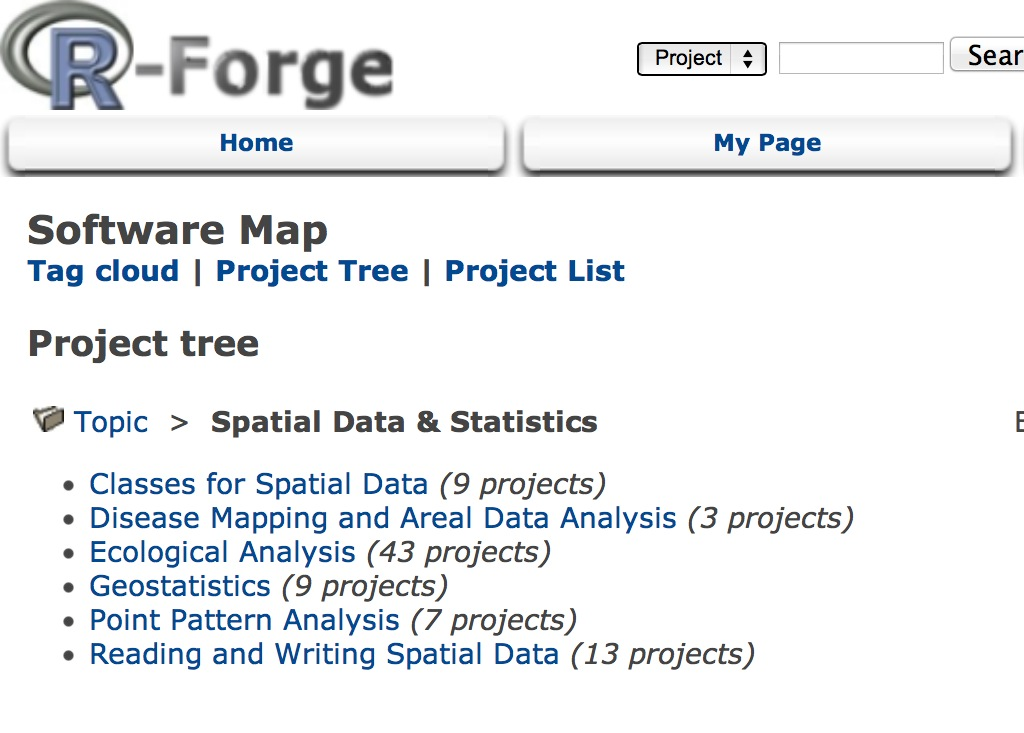
\includegraphics[width=0.8\textwidth]{Figures/Rforge.png}
\end{frame}

%------------------------------------------------

\begin{frame}
\frametitle{RSpatial}
\centering
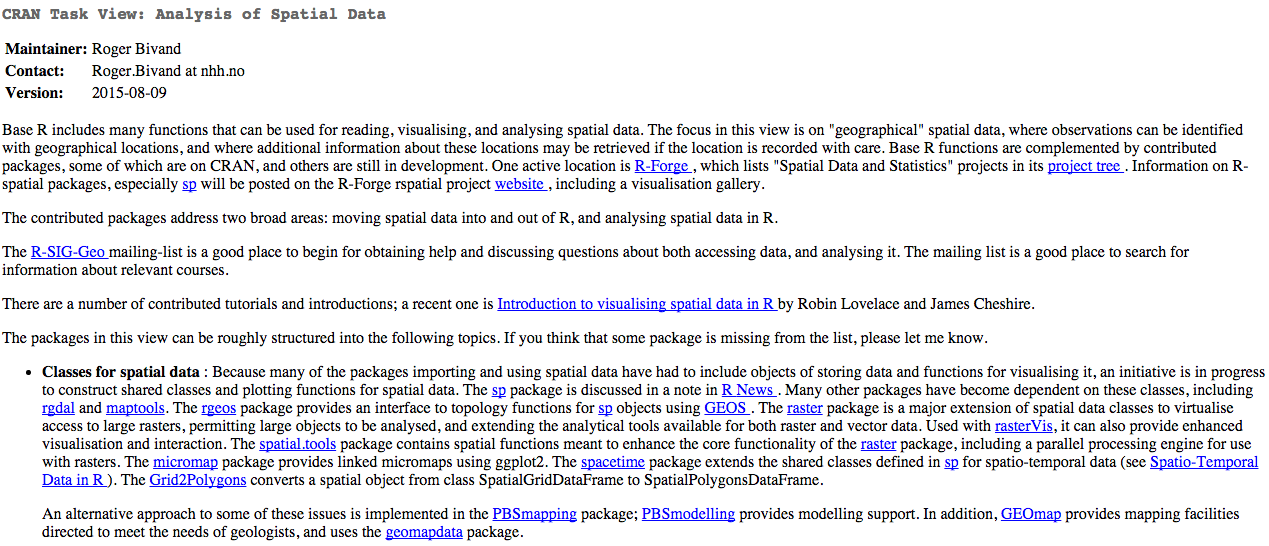
\includegraphics[width=\textwidth]{Figures/Rspatial.png}\\
\href{https://cran.r-project.org/web/views/Spatial.html}{https://cran.r-project.org/web/views/Spatial.html}
\end{frame}

%------------------------------------------------

\begin{frame}
\frametitle{R Cookbook}
\centering
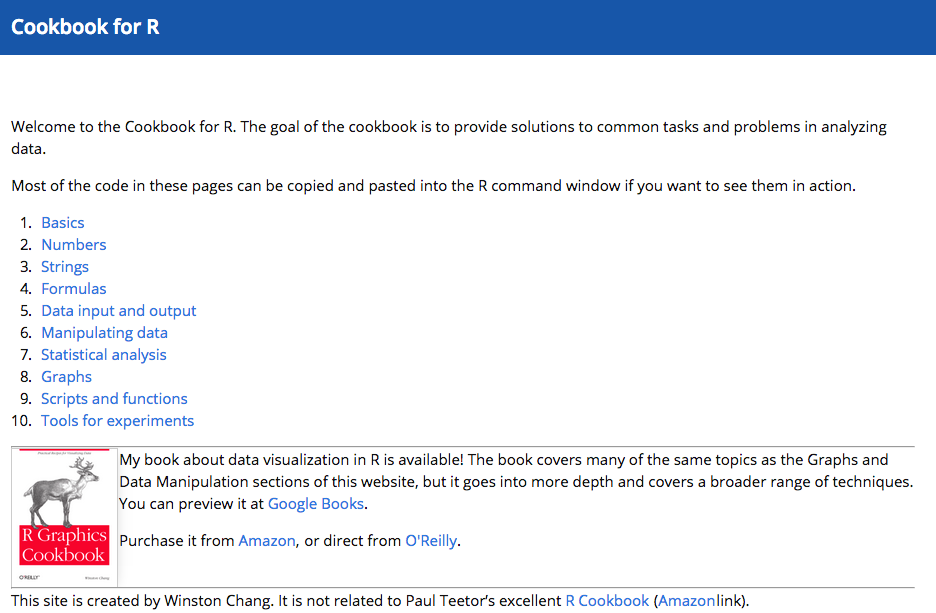
\includegraphics[width=0.9\textwidth]{Figures/cookbook.png}\\
\href{http://www.cookbook-r.com/}{http://www.cookbook-r.com/}
\end{frame}

%------------------------------------------------

\begin{frame}
\centering
The slides, scripts, materials and data are available from:\\
\href{https://github.com/AvitBhowmik/summer_academy_15}{\alert{https://github.com/AvitBhowmik/summer\textunderscore academy\textunderscore 15}}\\
\vspace{1cm}
\Huge See you on Monday!
\end{frame}

%------------------------------------------------

\end{document} 